\documentclass[aspectratio=169,
hyperref={colorlinks,urlcolor=blue}
]{beamer}


%\usetheme{Pittsburgh}
\usetheme{default}
\usepackage{colortbl}%colored tables
%For using helvetica font:
\usepackage[scaled]{helvet}
\usepackage[T1]{fontenc}
\renewcommand\familydefault{\sfdefault}
\urlstyle{same} %sets the fonts for urls
\usepackage{pdfpages}
\usepackage{siunitx}
\usepackage{caption}
\usepackage{pifont}%for dings
\usepackage{pgfplots}%for 3d plotting
\pgfplotsset{compat = newest}
\usepackage{mathtools}%box in align env \Aboxed
\usepackage[american,smartlabels]{circuitikz}%for drawing circuits
\usepackage{multimedia}
\usepackage{animate}
\usepackage{xcolor}


\usetikzlibrary{arrows}
\usetikzlibrary {3d} 
\usetikzlibrary{decorations.markings, math}
\usetikzlibrary{intersections, pgfplots.fillbetween}
\usetikzlibrary {shapes.geometric} 


%\definecolor{myblue}{RGB}{5, 34, 150}
\definecolor{myblue2}{RGB}{5, 34, 150}
\definecolor{myblue}{RGB}{0,36,82}
\definecolor{myred}{RGB}{207, 2, 13}
\definecolor{mygreen}{RGB}{0, 158, 11}
\definecolor{myyellow}{RGB}{220,220,0}
\definecolor{qblue}{RGB}{0,36,82}
\definecolor{qgold}{RGB}{250,189,15}
\definecolor{qred}{RGB}{185,14,49}
\definecolor{cblue}{rgb}{0.13, 0.67, 0.8}
\definecolor{corange}{rgb}{0.8, 0.34, 0.0}
\definecolor{cpurple}{rgb}{0.54, 0.29, 0.42}

%%%%%%%%%%%% General settings
\setbeamercolor{frametitle}{fg=black}
\setbeamercolor{title}{fg=black}
\setbeamercolor{author}{fg=myblue2}

\beamertemplatenavigationsymbolsempty %no navigation controls at bottom of slides
%\setbeamertemplate{footline}[frame number]
\usefonttheme{professionalfonts} 
\setbeamerfont{title}{series=\bfseries,parent=structure}
\setbeamerfont{frametitle}{series=\bfseries,parent=structure}

%%%%%%%%%%%%Lists
\setbeamertemplate{itemize item}[circle] %{\color{myblue}$\circ$}
\setbeamertemplate{itemize subitem}{\color{myblue2}$\circ$}
\setbeamertemplate{itemize subsubitem}{\color{myblue2}$\cdot$}
\setbeamercolor{itemize item}{bg=myblue2,fg=myblue2}
\setbeamercolor{enumerate item}{bg=myblue2,fg=myblue2}
%%%%%%%%%%%%%%%%%%%%%%%%%%%%

%%%%%%%%%%%%Blocks
\setbeamertemplate{blocks}[rounded]
%Default block
\setbeamercolor{block title}{bg=myblue2, fg=white}
\setbeamercolor{block body}{bg=myblue2!10}
\setbeamerfont{block body}{size=\scriptsize}
\setbeamerfont{block title}{size=\scriptsize}
%Alert block
\setbeamercolor{block title alerted}{bg= myblue2, fg=white}
\setbeamercolor{block body alerted}{bg=myblue2!10}
\setbeamerfont{block body alerted}{size=\scriptsize}
\setbeamerfont{block title alerted}{size=\scriptsize}
%example block
\setbeamercolor{block title example}{bg=mygreen, fg=white}
\setbeamercolor{block body example}{bg=mygreen!10}
\setbeamerfont{block body example}{size=\scriptsize}
\setbeamerfont{block title example}{size=\scriptsize}
%%%%%%%%%%%%%%%%55


%%%%%%%%%%%%Figures and captions
\captionsetup{font=scriptsize,labelfont=scriptsize}
%\setbeamertemplate{caption}{\raggedright\insertcaption\par}
\newenvironment{capfig}[3]{\begin{figure}\includegraphics[width=#1\textwidth]{#2}\caption*{\textit{#3}}\end{figure}}{}

%\makeatother
%\setbeamertemplate{footline}
%{
%  \leavevmode%
%  \hbox{%
%  \begin{beamercolorbox}[wd=.4\paperwidth,ht=2.25ex,dp=1ex,center]{author in head/foot}%
%    \usebeamerfont{author in head/foot}\insertshortauthor
%  \end{beamercolorbox}%
%  \begin{beamercolorbox}[wd=.6\paperwidth,ht=2.25ex,dp=1ex,center]{title in head/foot}%
%    \usebeamerfont{title in head/foot}\insertshorttitle\hspace*{3em}
%    \insertframenumber{} / \inserttotalframenumber\hspace*{1ex}
%  \end{beamercolorbox}
%  }%
%  \vskip0pt%
%}
%\makeatletter

\makeatother
\setbeamertemplate{footline}
{
  \leavevmode%
  \hbox{%
\begin{beamercolorbox}[wd=.27\paperwidth,ht=2.25ex,dp=1ex,center]{author in head/foot}%
    \color{black}{\insertinstitute}
\end{beamercolorbox}
  \begin{beamercolorbox}[wd=.27\paperwidth,ht=2.25ex,dp=1ex,center]{author in head/foot}%
    \color{black}{\inserttitle}
  \end{beamercolorbox}%
  \begin{beamercolorbox}[wd=.27\paperwidth,ht=2.25ex,dp=1ex,center]{title in head/foot}%
    \color{black}{\insertshortauthor}
  \end{beamercolorbox}
  \begin{beamercolorbox}[wd=.27\paperwidth,ht=2.25ex,dp=1ex,center]{title in head/foot}%
    \hspace{.28\paperwidth}\color{black} \insertframenumber{} / \inserttotalframenumber\hspace*{1ex}
  \end{beamercolorbox}
  }%
  \vskip0pt%
}
\makeatletter

\setbeamertemplate{title page}
{
  \begin{tikzpicture}[remember picture,overlay]
    \def\barh{4}%15
  
    \draw[color=myblue2,line width=\barh] ([yshift=-0.5*\barh]current page.north west) -- ([yshift=-0.5*\barh,xshift=-0.67\paperwidth]current page.north east);
    \draw[color=myblue2,line width=\barh] ([yshift=-0.5*\barh,xshift=-0.67\paperwidth]current page.north east) -- ([yshift=-0.5*\barh,xshift=-0.34\paperwidth]current page.north east);
    \draw[color=myblue2,line width=\barh] ([yshift=-0.5*\barh,xshift=-0.34\paperwidth]current page.north east) -- ([yshift=-0.5*\barh]current page.north east); 
  
    \draw[color=myblue2,line width=\barh] ([yshift=0.5*\barh]current page.south west) -- ([yshift=0.5*\barh,xshift=-0.67\paperwidth]current page.south east);
    \draw[color=myblue2,line width=\barh] ([yshift=0.5*\barh,xshift=-0.67\paperwidth]current page.south east) -- ([yshift=0.5*\barh,xshift=-0.34\paperwidth]current page.south east);
    \draw[color=myblue2,line width=\barh] ([yshift=0.5*\barh,xshift=-0.34\paperwidth]current page.south east) -- ([yshift=0.5*\barh]current page.south east);
    %\node[left] at (current page.east) {
    %
\includegraphics[scale=0.1]{figures/coverpage}
    %};
  \end{tikzpicture}
  
  \usebeamerfont{title}\usebeamercolor[fg]{title}\inserttitle\par
  \usebeamerfont{subtitle}\usebeamercolor[fg]{subtitle}\insertsubtitle\par
  \vspace{2cm}
  \usebeamerfont{author}\usebeamercolor[fg]{author}\insertauthor\par
  \usebeamerfont{institute}\usebeamercolor[fg]{author}\insertinstitute\par
  \usebeamercolor[fg]{author}\par
  \usebeamercolor[fg]{titlegraphic}\inserttitlegraphic

} 

\setbeamertemplate{frametitle}{%
    \nointerlineskip%
        \par\hspace*{-\dimexpr0.5\paperwidth-0.5\textwidth}\textcolor{myblue2}{\rule{0.33\paperwidth}{6pt}}\textcolor{myblue2}{\rule{0.33\paperwidth}{6pt}}\textcolor{myblue2}{\rule{0.34\paperwidth}{6pt}} 
    \begin{beamercolorbox}[wd=\paperwidth,ht=0.75cm,dp=0.6ex]{frametitle}
        \hspace*{0.5cm}\strut\usebeamerfont{frametitle}\insertframetitle\strut
        %\hrule
    \end{beamercolorbox}%
    %%Line below:
%\par\hspace*{-\dimexpr0.5\paperwidth-0.5\textwidth}\textcolor{myblue}{\rule{\paperwidth}{0.4pt}}
     % <-- calculation of left margin width + rule
     %\textcolor{red}{\noindent\rule{\paperwidth}{2pt}}
}


%%%%%%%%%%%%Frame templates

%Slide with title
\newenvironment{titleframe}[1]
{\begin{frame}\frametitle{#1}\end{frame}}
{}

%Slide with title and itemize list:
\newenvironment{bulletframe}[1]
{\begin{frame}{#1} \itemize}
{\enditemize \end{frame}}

%Slide with two columns 50/50
\newenvironment{twocolframe}[3]
{\begin{frame}{#1}
 \begin{columns}[T]
 \column{0.5\textwidth}#2
 \column{0.5\textwidth}#3
 \end{columns}\end{frame}}{}

%Slide with two columns 60/40 <<<<<<<<<<<<<<<<<<<<<<  This one!
\newenvironment{twocolframesf}[3]
{\begin{frame}{#1}
 \begin{columns}[T]
 \column{0.6\textwidth}#2
 \column{0.4\textwidth}#3
 \end{columns}\end{frame}}{}
 
%Slide with two columns 70/30
\newenvironment{twocolframest}[3]
{\begin{frame}{#1}
 \begin{columns}[T] 
 \column{0.7\textwidth}#2
 \column{0.3\textwidth}#3
 \end{columns}\end{frame}}{} 
 
%Slide with two columns 40/60
\newenvironment{twocolframefs}[3]
{\begin{frame}{#1}
 \begin{columns}[T] 
 \column{0.4\textwidth}#2
 \column{0.6\textwidth}#3
 \end{columns}\end{frame}}{}
 
%Slide with two columns 70/30
\newenvironment{twocolframets}[3]
{\begin{frame}{#1}
 \begin{columns}[T] 
 \column{0.3\textwidth}#2
 \column{0.7\textwidth}#3
 \end{columns}\end{frame}}{} 

 
%Colloquium speaker (title, abstract, picture file, speaker name)
\newenvironment{colloquium}[5]
{
\begin{frame}{Colloquium: Friday 1:30pm in Stirling A}
\begin{columns}[T] 
 \column{0.8\textwidth}
 \textbf{#1}\\
 #2
 \column{0.2\textwidth}
 \capfig{#3}{#4}{#5}
 \end{columns}
\end{frame}
}
{} 

%%%%%%%%%%%%%Set Hyperref colors


\hypersetup{
  colorlinks=true,
  linkcolor=blue,    
  urlcolor=blue,     
  citecolor=blue      
}
%%%%%%%%%%%%%TOC bolding
\setbeamerfont{section in toc}{series=\bfseries}



%Frames:
% \twocolframesf 60/40 (fs, st, ts) 
% \titleframe
% bulletframe


%%%%%%%%%%%%%%%%%%%%%%%%%
%%%%%% START OF PRESENTATION %%%%%%
%%%%%%%%%%%%%%%%%%%%%%%%%
\title{Current}
\subject{Electric Current, Ohm's Law, and Power}
\subtitle{Building Models to Describe our World}


%%%%%%%%%%%%%%%%%%%%%%%%%%%%%%
%%%%%%%%%%%%%%%%%%%%%



\begin{document}

%%%%%%%%%%%%%%%%%%%%%%%%%
%%%%%% Title slide %%%%%%
%%%%%%%%%%%%%%%%%%%%%%%%%
\chaptertitle{Current}
\begin{frame}
\titlepage
\thispagestyle{empty}

\begin{textblock*}{5cm}(11cm,4cm)
    
\includegraphics[width=4cm]{figures/BMDW/logo}
\end{textblock*}

\end{frame}

%%%%%%%%%%%%%TOC
\twocolframe{Outline}
  {\tableofcontents[sections={1,2}, subsectionstyle=show/show]\thispagestyle{empty}}
  {\tableofcontents[sections={3}, subsectionstyle=show/show]}
%%%%%%%%%%%%%%%%%%%%%%%%%







%%%%%%%%%%%%%%%%%%%%%%%%%%%%%%%%
\section{Electric Current}
\label{sec:electriccurrent}
\title{Electric Current}


%%%%%%%%%%%%%%%%%%%%%%%%%
\begin{frame}
\titlepage
\thispagestyle{empty}
\end{frame}

%%%%%%%%%%%%%%%%%%

\twocolframesf{Electric current}
{
\begin{itemize}
 \item Electric current is a measure of the rate at which charge flows through a material:
 \begin{align*}
 I = \frac{\Delta Q}{\Delta t}= \frac{dQ}{dt}
 \end{align*}
 \item Current is positive in the direction in which positive charges flow. In reality, it is \textbf{almost always electrons
that flow}, so current is usually in the \textit{opposite} direction of the flow of the actual charges.
 \item Electric current is a \textit{macroscopic} quantity. 
\end{itemize}
}
{
\centering
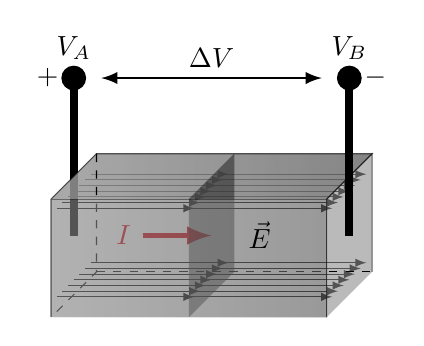
\begin{tikzpicture}[scale=0.5]
  \def\L{7.0}
  \def\h{3.0}
  \def\w{3.0}
  \def\H{4.0}
  
  %Electric field lines
  \begin{scope}[ decoration={
    markings,
    mark=at position 0.5 with {\arrow{latex}}}
    ] 
    
  \foreach \i in {1,...,7}
  {
    \draw[-latex,postaction={decorate}] (0,1/8*\h,-1/8*\i*\w) -- (\L,1/8*\h,-1/8*\i*\w);
    \draw[-latex,postaction={decorate}] (0,7/8*\h,-1/8*\i*\w) -- (\L,7/8*\h,-1/8*\i*\w);
  }

  \end{scope}
  
  %Current with arrow, first since needs to be "inside"
  \draw[line width=2pt,black, -latex,color=myred] (\L/4,\h/2,-\w/2) node[left] {$I$}  -- (\L/2,\h/2,-\w/2);  
  %Terminals: (The one on the left needs to be partially hidden)
  \draw[line width=3pt] (0, \h/2,-\w/2) --(0,\H+ \h/2,-\w/2) ;
  \draw[fill=black] (0,\H+ \h/2,-\w/2) circle (0.3)node[above=3pt] {$V_A$} node[left=2pt]{$+$};
  \draw[fill=black] (\L,\H+ \h/2,-\w/2) circle (0.3) node[above=3pt] {$V_B$}node[right=2pt]{$-$};
  \draw[line width=1pt,latex-latex] (\L/10,\H+ \h/2,-\w/2) -- (9*\L/10,\H+ \h/2,-\w/2) node[midway,above]{$\Delta V$};
  
  %Rectangle:
  \fill[left color=gray!30!,right color=gray!80,shading=axis,opacity=0.6, draw=black] (0,\h,0) -- (0,\h,-\w)--(\L,\h,-\w) -- (\L,\h,0);
  \fill[color=gray!90,opacity=0.6, draw=black] (\L,0,0) -- (\L,\h,0)--(\L,\h,-\w) -- (\L,0,-\w);
  %plane (inside)
  \fill[color=gray!20!black,opacity=0.5] (\L/2,0,0) -- (\L/2,\h,0)--(\L/2,\h,-\w) -- (\L/2,0,-\w);
  \draw[dashed] (0,\h,-\w) -- (0,0,-\w) -- (0,0,0);
  \draw[dashed] (0,0,-\w) -- (\L,0,-\w);
  %front face
  \fill[left color=gray!30!,right color=gray!80,shading=axis,opacity=0.4, draw=black] (0,0,0) -- (0,\h,0)--(\L,\h,0) -- (\L,0,0);
  %%%%%%%%%%% end of 3d rectangle

  %P

  \node[left] at (3/4*\L,\h/2,-\w/2) {$\vec E$} ;

  \draw[line width=3pt] (\L, \h/2,-\w/2) --(\L,\H+ \h/2,-\w/2) ;
  
 
  
\end{tikzpicture}
\captionof*{figure}{\textit{We apply a potential difference, $\Delta V$, across a metal and current, $I$, flows.}}

}



\def\proton at (#1,#2,#3){
\draw[fill=black,opacity=0.8] (#1,#2) circle (#3);
\node[text=white] at (#1,#2) {\tiny$+$};
\draw (#1+1.2*#3,#2) arc (0:90:1.2*#3);
\draw (#1+1.5*#3,#2) arc (0:90:1.5*#3);
\draw (#1+-1.2*#3,#2) arc (180:270:1.2*#3);
\draw (#1+-1.5*#3,#2) arc (180:270:1.5*#3);
}


%%%%%%%%%%%%%%%%%%%%%%%%%%%%%%
\subsection{Microscopic model of current}
\label{subsec:microscopicmodelofcurrent}
\twocolframesf{Microscopic model of current}
{
\begin{itemize}
 \item We can model current in a metal using a \textit{microscopic} model of charges ``drifting'' through the metal with an average velocity:
\begin{itemize}
 \item Typical \textbf{drift velocity}: $ v_d \sim \SI{1e-4}{m/s}$
 \end{itemize}
 \item In reality, electrons are moving around much faster, in mostly random directions and bouncing off of atoms:
\begin{itemize}
 \item Typical speed of electrons: \SI{1e8}{m/s}
 \end{itemize}
\end{itemize}
}
{
\centering

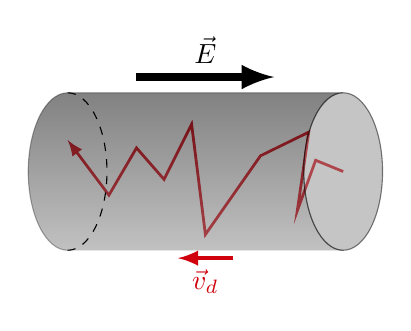
\begin{tikzpicture}[scale=0.5]
  \def\L{7.0}
  \def\R{2}
  \def\pr{0.25}
  
  %\proton at (0,3,0.25);

\proton at (0,0.7*\R,\pr);
\proton at (0,-0.7*\R,\pr);
\proton at (0,0,\pr);
\proton at (\L/10,0.35*\R,0.8*\pr);
\proton at (\L/10,-0.35*\R,0.8*\pr);
\proton at (0.2*\L,0,\pr);
\proton at (0.2*\L,0.7*\R,\pr);
\proton at (0.2*\L,-0.7*\R,\pr);
\proton at (0.3*\L,0.35*\R,1.2*\pr);
\proton at (0.3*\L,-0.35*\R,1.2*\pr);
\proton at (0.4*\L,0,\pr);
\proton at (0.4*\L,0.7*\R,\pr);
\proton at (0.4*\L,-0.7*\R,\pr);
\proton at (0.5*\L,0.35*\R,0.8*\pr);
\proton at (0.5*\L,-0.35*\R,0.8*\pr);
\proton at (0.6*\L,0,\pr);
\proton at (0.6*\L,0.7*\R,\pr);
\proton at (0.6*\L,-0.7*\R,\pr);
\proton at (0.7*\L,0.35*\R,1.2*\pr);
\proton at (0.7*\L,-0.35*\R,1.2*\pr);
\proton at (0.8*\L,0,\pr);
\proton at (0.8*\L,0.7*\R,\pr);
\proton at (0.8*\L,-0.7*\R,\pr);
\proton at (0.9*\L,0.35*\R,0.8*\pr);
\proton at (0.9*\L,-0.35*\R,0.8*\pr);
\proton at (\L,0,\pr);
\proton at (\L,0.7*\R,\pr);
\proton at (\L,-0.7*\R,\pr);

\draw[line width=1pt,-latex,color=myred] (\L,0) -- (\L-\L/10,\R/7) -- (\L-\L/6,-\R/2) --  (\L-\L/8,\R/2) -- (0.7*\L,0.2*\R) -- (0.5*\L,-0.8*\R)-- (0.45*\L,0.6*\R)-- (0.35*\L,-0.1*\R)-- (0.25*\L,0.3*\R)-- (0.15*\L,-0.3*\R)-- (0.,0.4*\R);
%cylinder:
  \fill[top color=gray!15!black,bottom color=gray!20,shading=axis,opacity=0.3, draw=black] (0,-\R) arc (270:90:\R/2 and \R) --  (0,\R)-- (\L, \R) arc (90:270:\R/2 and \R) -- (\L,-\R); 
  \draw[dashed] (0,\R) arc (90:-90:\R/2 and \R) ;
  \fill[color=gray!90,opacity=0.5,draw=black] (\L+\R/2, 0) arc (0:360:\R/2 and \R);
  %%%%%%%%%%
  %\draw[line width=1pt,latex-latex] (0,-1.1*\R) -- (\L,-1.1*\R) node[midway,below]{$\Delta V,L$};
  \draw[line width=3pt,-latex] (\L/4,1.2*\R) -- (3*\L/4,1.2*\R) node[midway,above]{$\vec E$};
  \draw[line width=1.5pt,color=myred,latex-] (0.4*\L,-1.1*\R) -- (0.6*\L,-1.1*\R) node[below, midway]{$\vec v_d$};
\end{tikzpicture}
\captionof*{figure}{\textit{An electron moving through a resistor and colliding with atoms, resulting in heat. The average speed of the electron is constant as the work done by the electric field is converted into heat.}}
}

%%%%%%%%%%%%%%%%%%%%%%%%%%%%%%
\def\electron at (#1,#2,#3){
\fill[color=myred,opacity=0.8] (#1,#2) circle (#3);
\draw[color=white] (#1-0.8*#3,#2) -- (#1+0.8*#3,#2); %- sign
\draw[color=myred,latex-] (#1-5*#3,#2) -- (#1-#3,#2);
}

\subsection{Drift velocity}
\label{subsec:driftvelocity}
\twocolframesf{Current and drift velocity}
{
We have, $n$, electrons per unit volume, with charge $q$, moving with average speed, $v_d$, through a resistor of cross-section, $A$: 
 \begin{itemize}
 \item<1-> In time $\Delta t$, electrons move a distance $l=v_d\Delta t$.
 \item<2-> This corresponds to a volume of electrons, $V=lA=v_d\Delta t A$
 \item<3-> with a total charge, $\Delta Q = Vnq = v_d\Delta t A nq$
 \item<4-> resulting in a current, $I$:\\
 $I=\frac{\Delta Q}{\Delta t}=v_d A nq$
 \end{itemize}
\only<5->{This allows us to relate a macroscopic quantity ($I$, current) to microscopic quantities (e.g. $v_d$).}
}
{
\centering

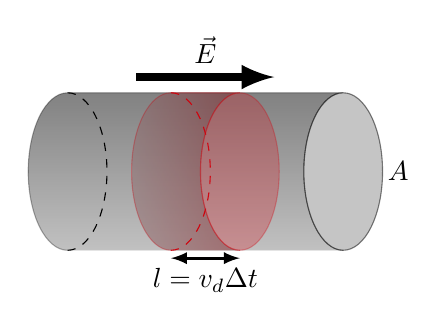
\begin{tikzpicture}[scale=0.5]
  \def\L{7.0}
  \def\R{2}
  \def\pr{0.15}
  
\electron at (0,0.7*\R,\pr);
\electron at (0,-0.7*\R,\pr);
\electron at (0,0,\pr);
\electron at (\L/10,0.35*\R,0.8*\pr);
\electron at (\L/10,-0.35*\R,0.8*\pr);
\electron at (0.2*\L,0,\pr);
\electron at (0.2*\L,0.7*\R,\pr);
\electron at (0.2*\L,-0.7*\R,\pr);
\electron at (0.3*\L,0.35*\R,1.2*\pr);
\electron at (0.3*\L,-0.35*\R,1.2*\pr);
\electron at (0.4*\L,0,\pr);
\electron at (0.4*\L,0.7*\R,\pr);
\electron at (0.4*\L,-0.7*\R,\pr);
\electron at (0.5*\L,0.35*\R,0.8*\pr);
\electron at (0.5*\L,-0.35*\R,0.8*\pr);
\electron at (0.6*\L,0,\pr);
\electron at (0.6*\L,0.7*\R,\pr);
\electron at (0.6*\L,-0.7*\R,\pr);
\electron at (0.7*\L,0.35*\R,1.2*\pr);
\electron at (0.7*\L,-0.35*\R,1.2*\pr);
\electron at (0.8*\L,0,\pr);
\electron at (0.8*\L,0.7*\R,\pr);
\electron at (0.8*\L,-0.7*\R,\pr);
\electron at (0.9*\L,0.35*\R,0.8*\pr);
\electron at (0.9*\L,-0.35*\R,0.8*\pr);
\electron at (\L,0,\pr);
\electron at (\L,0.7*\R,\pr);
\electron at (\L,-0.7*\R,\pr);

%cylinder:
  \fill[top color=gray!15!black,bottom color=gray!20,shading=axis,opacity=0.3, draw=black] (0,-\R) arc (270:90:\R/2 and \R) --  (0,\R)-- (\L, \R) arc (90:270:\R/2 and \R) -- (\L,-\R); 
  \draw[dashed] (0,\R) arc (90:-90:\R/2 and \R) ;
  \fill[color=gray!90,opacity=0.5,draw=black] (\L+\R/2, 0) arc (0:360:\R/2 and \R);
%%%%%%  
   \fill[left color=myred!30!,right color=myred!80,shading=axis,opacity=0.3, draw=myred] (3*\L/8,-\R) arc (270:90:\R/2 and \R) --  (3*\L/8,\R)-- (5*\L/8, \R) arc (90:270:\R/2 and \R) -- (5*\L/8,-\R); 
  \draw[dashed,color=myred] (3*\L/8,\R) arc (90:-90:\R/2 and \R) ;
  \fill[color=myred!90,opacity=0.3,draw=myred] (5*\L/8+\R/2, 0) arc (0:360:\R/2 and \R);  
%%%%%%%%%%%%%%55 
  \node at (1.2*\L,0) {$A$};
  \draw[line width=1pt,latex-latex] (3*\L/8,-1.1*\R) -- (5*\L/8,-1.1*\R) node[midway,below]{$l=v_d\Delta t$};
  \draw[line width=3pt,-latex] (\L/4,1.2*\R) -- (3*\L/4,1.2*\R) node[midway,above]{$\vec E$};
\end{tikzpicture}
\captionof*{figure}{\textit{Electrons drifting with an average velocity, $\vec v_d$}}
}

%%%%%%%%%%%%%%%%%%%%%%%%%%%%%%
\twocolframesf{Current and current density}
{
\begin{itemize}
 \item We can model charges moving through a metal macroscopically, by using current, $I$:
\begin{align*}
I = \frac{dQ}{dt}
\end{align*}
This is the amount of charge flowing through cross section, $A$, of the metal per unit time.
 \item We can define the current density, as the current per unit area, $j$:
\begin{align*}
j = \frac{I}{A}
\end{align*}
$j$, the current density can depend on position and is a microscopic quantity.
\end{itemize}

}
{
\centering

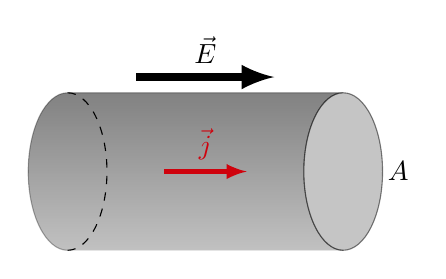
\begin{tikzpicture}[scale=0.5]
  \def\L{7.0}
  \def\R{2}
  \def\pr{0.15}
  
%cylinder:
  \fill[top color=gray!15!black,bottom color=gray!20,shading=axis,opacity=0.3, draw=black] (0,-\R) arc (270:90:\R/2 and \R) --  (0,\R)-- (\L, \R) arc (90:270:\R/2 and \R) -- (\L,-\R); 
  \draw[dashed] (0,\R) arc (90:-90:\R/2 and \R) ;
  \fill[color=gray!90,opacity=0.5,draw=black] (\L+\R/2, 0) arc (0:360:\R/2 and \R);
%%%%%%  
 
  \node at (1.2*\L,0) {$A$};

  \draw[line width=3pt,-latex] (\L/4,1.2*\R) -- (3*\L/4,1.2*\R) node[midway,above]{$\vec E$};
  \draw[line width=1.5pt,color=myred,-latex] (0.35*\L,0) -- (0.65*\L,0) node[above, midway]{$\vec j$};
\end{tikzpicture}
\captionof*{figure}{\textit{Current density is a vector parallel to the electric field (and anti-parallel to drift velocity for electrons).}}
}

%%%%%%%%%%%%%%%%%%%%%%%%%%%%%%
\subsection{Current density}
\label{subsec:currentdensity}
\subsubsection{At the microscopic level}
\label{subsubsec:atthemicroscopiclevel}
\twocolframesf{Current density at the microscopic level}
{
\begin{itemize}
 \item We define the \textbf{current density, $\vec j$, as a vector parallel to the electric field}, corresponding to the direction of the average flow of positive charges.
\item If we choose a surface, the current through that surface is that part of the current density flowing perpendicular to the surface:
\begin{align*}
I = \int \vec j \cdot d\vec A=\int j dA_\perp
\end{align*}
(just like a ``flux''; in fact, exactly a flux!)
\end{itemize}
}
{
\centering

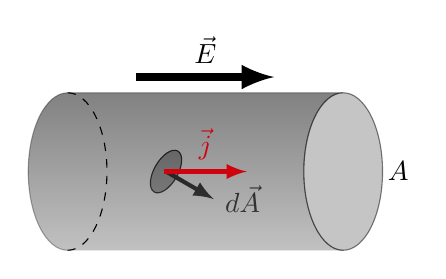
\begin{tikzpicture}[scale=0.5]
  \def\L{7.0}
  \def\R{2}
  \def\pr{0.15}
  
  \begin{scope}[xshift=2.5cm, rotate=-30]
  \fill[color=gray!80,draw=black] (0.,0) ellipse(0.15*\R/1 and 0.3*\R);
  \draw[line width=1.5pt,color=black,-latex] (0,0) -- (0.2*\L,0) node[right]{$d\vec A$};
  \end{scope}
  
%cylinder:
  \fill[top color=gray!15!black,bottom color=gray!20,shading=axis,opacity=0.3, draw=black] (0,-\R) arc (270:90:\R/2 and \R) --  (0,\R)-- (\L, \R) arc (90:270:\R/2 and \R) -- (\L,-\R); 
  \draw[dashed] (0,\R) arc (90:-90:\R/2 and \R) ;
  \fill[color=gray!90!,opacity=0.5,draw=black] (\L+\R/2, 0) arc (0:360:\R/2 and \R);
%%%%%%  
 
  \node at (1.2*\L,0) {$A$};

  \draw[line width=3pt,-latex] (\L/4,1.2*\R) -- (3*\L/4,1.2*\R) node[midway,above]{$\vec E$};
  \draw[line width=1.5pt,color=myred,-latex] (0.35*\L,0) -- (0.65*\L,0) node[above, midway]{$\vec j$};
\end{tikzpicture}
\captionof*{figure}{\textit{Current density is a vector parallel to the electric field (and anti-parallel to drift velocity for electrons).}}
}


%%%%%%%%%%%%%%%%%%%%%%%%%%%%%%
\subsubsection{From drift velocity}
\label{subsubsec:fromdriftvelocity}
\begin{bulletframe}{Current density from drift velocity}
\item The current:
\begin{align*}
\vec I = -enA\vec v_d
\end{align*}
\item The current density:
\begin{align*}
\vec j= \frac{\vec I}{A} = -en\vec v_d
\end{align*}
Here, we have explicitly chosen negative charges (electrons with charge $q=-e=\SI{-1.6e-19}{C}$). Current and current density are in the opposite direction of the drift velocity because $q$ is negative.
\end{bulletframe}

%%%%%%%%%%%%%%%%%%%%%%%%%%%%%%





\section{Ohm's Law}
\label{sec:ohmslaw}
\title{Ohm's Law}


%%%%%%%%%%%%%%%%%%%%%%%%%
\begin{frame}
\titlepage
\thispagestyle{empty}
\end{frame}





%%%%%%%%%%%%%%%%%%%%%%%%%%%%
\begin{bulletframe}{Ohm's Law}
\item For most materials:
\begin{align*}
\vec j= \sigma \vec E
\end{align*}
(We call these ``ohmic'' materials, because the law holds).
\item $\sigma$ is the \textbf{conductivity} of the material; it is a material-dependent measure of how large a current density one gets for a given applied electric field.
\end{bulletframe}


%%%%%%%%%%%%%%%%%%%%%%%%%%%%%%
\subsection{Macroscopically}
\label{subsec:macroscopically}
\twocolframesf{Ohm's Law, macroscopically}
{
\begin{itemize}
\item Microscopically:
\begin{align*}
\vec j= \frac{\vec I}{A} = -en\vec v_d\;\;\;\;\vec j = \sigma\vec E
\end{align*}
\item Relation between current and current density, on a \textit{macroscopic} piece of metal: 
\begin{align*}
\frac{I}{A} &= \sigma E=\sigma \frac{\Delta V}{L}\\
\only<1>{
\therefore \Delta V &= \frac{1}{\sigma}\frac{L}{A}I\\
}
\only<2>{
\therefore \Delta V &= \textcolor{myred}{\frac{1}{\sigma}\frac{L}{A}}I\\
\Aboxed{\Delta V &=\textcolor{myred}{R} I}
}
\end{align*}
\end{itemize}
}
{
\only<1>{
\centering
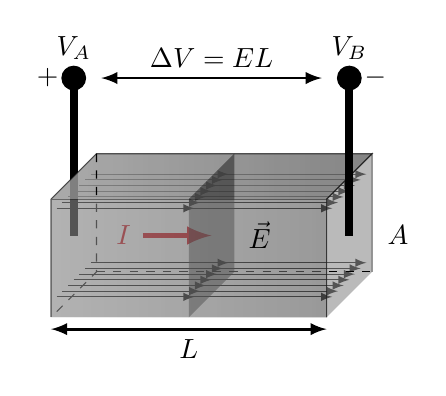
\begin{tikzpicture}[scale=0.5]
  \def\L{7.0}
  \def\h{3.0}
  \def\w{3.0}
  \def\H{4.0}
  
  %Electric field lines
  \begin{scope}[ decoration={
    markings,
    mark=at position 0.5 with {\arrow{latex}}}
    ] 
    
  \foreach \i in {1,...,7}
  {
    \draw[-latex,postaction={decorate}] (0,1/8*\h,-1/8*\i*\w) -- (\L,1/8*\h,-1/8*\i*\w);
    \draw[-latex,postaction={decorate}] (0,7/8*\h,-1/8*\i*\w) -- (\L,7/8*\h,-1/8*\i*\w);
  }

  \end{scope}
  
  %Current with arrow, first since needs to be "inside"
  \draw[line width=2pt,black, -latex,color=myred] (\L/4,\h/2,-\w/2) node[left] {$I$}  -- (\L/2,\h/2,-\w/2);  
  %Terminals: (The one on the left needs to be partially hidden)
  \draw[line width=3pt] (0, \h/2,-\w/2) --(0,\H+ \h/2,-\w/2) ;
  \draw[fill=black] (0,\H+ \h/2,-\w/2) circle (0.3)node[above=3pt] {$V_A$} node[left=2pt]{$+$};
  \draw[fill=black] (\L,\H+ \h/2,-\w/2) circle (0.3) node[above=3pt] {$V_B$}node[right=2pt]{$-$};
  \draw[line width=1pt,latex-latex] (\L/10,\H+ \h/2,-\w/2) -- (9*\L/10,\H+ \h/2,-\w/2) node[midway,above]{$\Delta V=EL$};
  
  %Rectangle:
  \fill[left color=gray!30!,right color=gray!80,shading=axis,opacity=0.6, draw=black] (0,\h,0) -- (0,\h,-\w)--(\L,\h,-\w) -- (\L,\h,0);
  \fill[color=gray!90,opacity=0.6, draw=black] (\L,0,0) -- (\L,\h,0)--(\L,\h,-\w) -- (\L,0,-\w);
  %plane (inside)
  \fill[color=gray!20!black,opacity=0.5] (\L/2,0,0) -- (\L/2,\h,0)--(\L/2,\h,-\w) -- (\L/2,0,-\w);
  \draw[dashed] (0,\h,-\w) -- (0,0,-\w) -- (0,0,0);
  \draw[dashed] (0,0,-\w) -- (\L,0,-\w);
  %front face
  \fill[left color=gray!30!,right color=gray!80,shading=axis,opacity=0.4, draw=black] (0,0,0) -- (0,\h,0)--(\L,\h,0) -- (\L,0,0);
  %%%%%%%%%%% end of 3d rectangle

  %Some labels
  \node[left] at (3/4*\L,\h/2,-\w/2) {$\vec E$} ;
  \draw[line width=3pt] (\L, \h/2,-\w/2) --(\L,\H+ \h/2,-\w/2) ;
  \draw[line width=1pt,latex-latex] (0,-\h/10,0) -- (\L,-\h/10,0) node[midway,below]{$L$};
  \node[left] at (1.25*\L,\h/2,-\w/2) {$A$} ;
  
\end{tikzpicture}
\captionof*{figure}{\textit{We apply a potential difference, $\Delta V$, across a metal and current, $I$, flows due to the electric field, $\vec E$.}}
}
\only<2>{
\begin{block}{Resistance}

We call, $R$, the ``resistance'' of the piece of material (a ``resistor''). 
\begin{align*}
R=\frac{1}{\sigma}\frac{L}{A}=\rho\frac{L}{A}
\end{align*}
where $\rho$ is the ``resistivity'' and $\sigma$ the ``conductivity'' of the material.\\
\textbf{Resistance} is the macroscopic property of resistor of length, $L$, area, $A$, made from a material with resistivity, $\rho$.
\end{block}
}

}


%%%%%%%%%%%%%%%%%%%%%%%%%%%%%%





%%%%%%%%%%%%%%%%%%%%%%%
\twocolframesf{Ohm's Law}
{
%\vspace{-1.5cm}
\begin{itemize}
\item Technically, Ohm’s Law refers to the microscopic version, $\vec j=\sigma \vec E$.
\item Ohm noted that the current through a material is proportional to the electric potential difference, introducing ``resistance'', $R$, as the constant of proportionality:
\begin{align*}
\Delta V \propto I= R I
\end{align*}
\item  For any ``resistor'' can use Ohm’s Law to find the current through it, given a potential difference.
\item High resistance $=$ low current for a given electric field
\end{itemize}


}
{
}

%%%%%%%%%%%%%%%%%%%%%%%%%%%%%%






%%%%%%%%%%%%%%%%%%%%%%%%%%%%%%5

\subsection{Resistance}
\label{subsec:resistance}
\twocolframesf{Resistance}
{
\begin{itemize}
\item Ohm's law for a resistor:
\begin{align*}
\Delta V = R I
\end{align*}
\item The resistance depends on the shape, $(L,A)$, and the material, $\rho$:
\begin{align*}
R=\rho\frac{L}{A}
\end{align*}
\only<2>{
\item Recall Poiseuille flow (fluid with viscosity):
\begin{align*}
\Delta P = R Q
\end{align*}
\item For a horizontal pipe: $R=\frac{8\eta L}{\pi r^4}$
}
\end{itemize}

}
{
\centering
\only<1>{
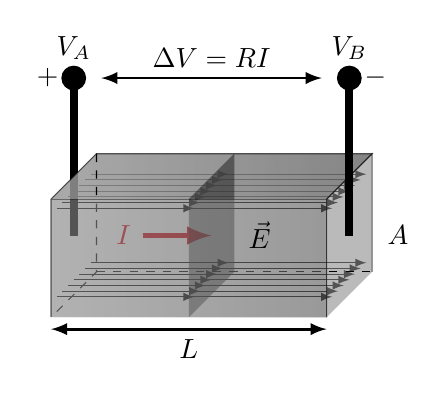
\begin{tikzpicture}[scale=0.5]
  \def\L{7.0}
  \def\h{3.0}
  \def\w{3.0}
  \def\H{4.0}
  
  %Electric field lines
  \begin{scope}[ decoration={
    markings,
    mark=at position 0.5 with {\arrow{latex}}}
    ] 
    
  \foreach \i in {1,...,7}
  {
    \draw[-latex,postaction={decorate}] (0,1/8*\h,-1/8*\i*\w) -- (\L,1/8*\h,-1/8*\i*\w);
    \draw[-latex,postaction={decorate}] (0,7/8*\h,-1/8*\i*\w) -- (\L,7/8*\h,-1/8*\i*\w);
  }

  \end{scope}
  
  %Current with arrow, first since needs to be "inside"
  \draw[line width=2pt,black, -latex,color=myred] (\L/4,\h/2,-\w/2) node[left] {$I$}  -- (\L/2,\h/2,-\w/2);  
  %Terminals: (The one on the left needs to be partially hidden)
  \draw[line width=3pt] (0, \h/2,-\w/2) --(0,\H+ \h/2,-\w/2) ;
  \draw[fill=black] (0,\H+ \h/2,-\w/2) circle (0.3)node[above=3pt] {$V_A$} node[left=2pt]{$+$};
  \draw[fill=black] (\L,\H+ \h/2,-\w/2) circle (0.3) node[above=3pt] {$V_B$}node[right=2pt]{$-$};
  \draw[line width=1pt,latex-latex] (\L/10,\H+ \h/2,-\w/2) -- (9*\L/10,\H+ \h/2,-\w/2) node[midway,above]{$\Delta V=RI$};
  
  %Rectangle:
  \fill[left color=gray!30!,right color=gray!80,shading=axis,opacity=0.6, draw=black] (0,\h,0) -- (0,\h,-\w)--(\L,\h,-\w) -- (\L,\h,0);
  \fill[color=gray!90,opacity=0.6, draw=black] (\L,0,0) -- (\L,\h,0)--(\L,\h,-\w) -- (\L,0,-\w);
  %plane (inside)
  \fill[color=gray!20!black,opacity=0.5] (\L/2,0,0) -- (\L/2,\h,0)--(\L/2,\h,-\w) -- (\L/2,0,-\w);
  \draw[dashed] (0,\h,-\w) -- (0,0,-\w) -- (0,0,0);
  \draw[dashed] (0,0,-\w) -- (\L,0,-\w);
  %front face
  \fill[left color=gray!30!,right color=gray!80,shading=axis,opacity=0.4, draw=black] (0,0,0) -- (0,\h,0)--(\L,\h,0) -- (\L,0,0);
  %%%%%%%%%%% end of 3d rectangle

  %Some labels
  \node[left] at (3/4*\L,\h/2,-\w/2) {$\vec E$} ;
  \draw[line width=3pt] (\L, \h/2,-\w/2) --(\L,\H+ \h/2,-\w/2) ;
  \draw[line width=1pt,latex-latex] (0,-\h/10,0) -- (\L,-\h/10,0) node[midway,below]{$L$};
  \node[left] at (1.25*\L,\h/2,-\w/2) {$A$} ;
  
\end{tikzpicture}
\captionof*{figure}{\textit{We apply a potential difference, $\Delta V$, across a resistor, $R$, and current, $I$, flows.}}
}

\only<2>{
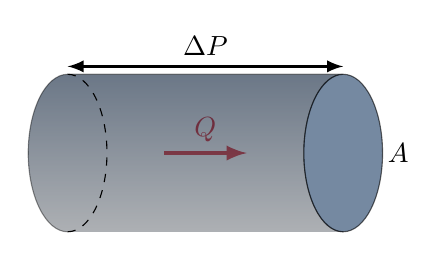
\begin{tikzpicture}[scale=0.5]
  \def\L{7.0}
  \def\R{2}
  \def\pr{0.15}
  
  \draw[line width=1.5pt,color=myred,-latex] (0.35*\L,0) -- (0.65*\L,0) node[above, midway]{$Q$};
    
%cylinder:
  \fill[top color=myblue!85,bottom color=myblue!20,shading=axis,opacity=0.4, draw=black] (0,-\R) arc (270:90:\R/2 and \R) --  (0,\R)-- (\L, \R) arc (90:270:\R/2 and \R) -- (\L,-\R); 
  \draw[dashed] (0,\R) arc (90:-90:\R/2 and \R) ;
  \fill[color=myblue!90,opacity=0.6,draw=black] (\L+\R/2, 0) arc (0:360:\R/2 and \R);
%%%%%%  
 
  \node at (1.2*\L,0) {$A$};
  \draw[line width=1pt,latex-latex] (0,1.1*\R) -- (\L,1.1*\R) node[midway,above]{$\Delta P$};

\end{tikzpicture}
\captionof*{figure}{\textit{A fluid flowing through a pipe due to a pressure difference.}}
\begin{exampleblock}{Analogy}
The math for current flowing through a resistor is the same as for fluid flowing through a pipe! Voltage is like pressure difference. 
\end{exampleblock}
}
}



%%%%%%%%%%%%%%%%%%%%%%%%%%%%%%




%%%%%%%%%%%%%%%%%%%%%%%%%%%%%%
\subsection{Combining resistors}
\label{subsec:combiningresistors}
\twocolframe{Combining resistors}
{
\only<1>{
\textbf{In series:} The voltages across each resistor add up to the battery voltage:
 \begin{align*}
 \Delta V_1 + \Delta V_2 &=\Delta V\\
  R_1I+R_2I&=R_{eff}I
 \end{align*}
Like making a longer resistor, total resistance increases:
\begin{align*}
R_{eff}=R_1+R_2
\end{align*} 
}
\only<2>{
\textbf{In parallel:} The currents through each resistor add up to the current through the battery:
 \begin{align*}
 I_1+I_2&= I\\
 \frac{\Delta V}{R_1}+\frac{\Delta V}{R_1}&= \frac{\Delta V}{R_{eff}}
 \end{align*}

Like making a wider resistor, total resistance decreases:
\begin{align*}
\frac{1}{R_{eff}}=\frac{1}{R_1}+\frac{1}{R_2}
\end{align*}
}
}
{
\begin{center}
\begin{tikzpicture}
\tikzmath{
\L=6;
\Lh=0.75;
\termh=0.25;
\h=1.5;
\Rh=0.75;
\Rl=0.35*\L;
\wl=(\L-3*\termh-2*\Rl)/3;
\wlp=(\L-3*\termh-\Rl)/2;
}
\scalebox{1}{
%battery and terminals:
\coordinate (T1) at (1.5*\termh,\termh);
\coordinate (T2) at (\L-1.5*\termh,\termh);

\fill[color=myblue!30,rounded corners] (0,-\Lh) rectangle (\L,0);
\fill[color=myblue!60] (\termh,0) rectangle +(\termh,\termh);
\fill[color=myblue!60] (\L-\termh,0) rectangle +(-\termh,\termh);
\node[below] at ($(T1)+((0,-\termh)$){$+$};
\node[below] at ($(T2)+((0,-\termh)$){$-$};
\draw[latex-latex] ($(T1)+(0,0.1)$) -- ($(T2)+(0,0.1)$) node[midway,above]{$\Delta V$};

%wires and resistors
\only<1>{
\draw[line width = 2] (T1) -- ($(T1)+(0,\h)$) -- ($(T1)+(\wl,\h)$);
\fill[color=myblue!30,rounded corners] ($(T1)+(\wl,\h-0.5*\Rh)$) rectangle +(\Rl,\Rh);
\draw[line width = 2] ($(T1)+(\wl+\Rl,\h)$) -- +(\wl,0);
\fill[color=myblue!30,rounded corners] ($(T1)+(2*\wl+\Rl,\h-0.5*\Rh)$) rectangle +(\Rl,\Rh);
\draw[line width = 2] ($(T1)+(2*\wl+2*\Rl,\h)$) -- +(\wl,0) -- (T2);

\node at ($(T1)+(\wl+\Rl/2,\h)$){$R_1$};
\node at ($(T1)+(2*\wl+1.5*\Rl,\h)$){$R_2$};

\draw[latex-latex] ($(T1)+(\wl,\h+0.5*\Rh+0.1)$) -- +(\Rl,0) node[midway,above]{$\Delta V_1=R_1I$};
\draw[latex-latex] ($(T1)+(2*\wl+\Rl,\h+0.5*\Rh+0.1)$) -- +(\Rl,0) node[midway,above]{$\Delta V_2=R_2I$};

\draw[-latex,line width=2, color=myred] ($(T1)+(0,0.4*\h)$) -- +(0,0.2*\h) node[left]{$I$};
\draw[-latex,line width=2, color=myred] ($(T2)+(0,0.6*\h)$) -- +(0,-0.2*\h) node[right]{$I$}; 
\draw[-latex,line width=2, color=myred] ($(T1)+(\wl+\Rl,\h)$) -- +(1.2*\wl,0) node[midway,below]{$I$};

\draw[dotted,line width=2, color=myblue!80] ($(T1)+(0.5*\wl,0.5*\h)$) rectangle +(2*\Rl+2*\wl,1.3*\h);
\node[above=5pt, color=myblue!80] at (0.5*\L,1.8*\h){$R_{eff}$};
}

\only<2>{
\draw[line width = 2] (T1) -- ($(T1)+(0,\h)$) -- ($(T1)+(\wlp,\h)$);
\fill[color=myblue!30,rounded corners] ($(T1)+(\wlp,\h-0.5*\Rh)$) rectangle +(\Rl,\Rh);
\draw[line width = 2] ($(T1)+(\wlp+\Rl,\h)$) -- +(\wlp,0) -- (T2);
\node at (\L/2,\termh+\h){$R_1$};
\draw[latex-latex] ($(T1)+(\wlp,\h+0.5*\Rh+0.1)$) -- +(\Rl,0) node[midway,above]{$\Delta V_1=R_1I_1$};


\draw[line width = 2] (T1) -- ($(T1)+(0,2*\h)$) -- ($(T1)+(\wlp,2*\h)$);
\fill[color=myblue!30,rounded corners] ($(T1)+(\wlp,2*\h-0.5*\Rh)$) rectangle +(\Rl,\Rh);
\draw[line width = 2] ($(T1)+(\wlp+\Rl,2*\h)$) -- +(\wlp,0) -- (T2);
\node at (\L/2,\termh+2*\h){$R_2$};
\draw[latex-latex] ($(T1)+(\wlp,2*\h+0.5*\Rh+0.1)$) -- +(\Rl,0) node[midway,above]{$\Delta V_2=R_2I_2$};

\draw[-latex,line width=2, color=myred] ($(T1)+(0,0.4*\h)$) -- +(0,0.2*\h) node[left]{$I$};
\draw[-latex,line width=2, color=myred] ($(T2)+(0,0.6*\h)$) -- +(0,-0.2*\h) node[right]{$I$}; 

\draw[-latex,line width=2, color=myred] ($(T1)+(0.4*\wlp,\h)$) -- +(0.2*\wlp,0) node[below]{$I_1$};
\draw[-latex,line width=2, color=myred] ($(T1)+(0.4*\wlp,2*\h)$) -- +(0.2*\wlp,0) node[below]{$I_2$};
\draw[-latex,line width=2, color=myred] ($(T1)+(1.4*\wlp+\Rl,\h)$) -- +(0.2*\wlp,0) node[below]{$I_1$};
\draw[-latex,line width=2, color=myred] ($(T1)+(1.4*\wlp+\Rl,2*\h)$) -- +(0.2*\wlp,0) node[below]{$I_2$};

\draw[dotted,line width=2, color=myblue!80] ($(T1)+(0.75*\wlp,0.5*\h)$) rectangle +(\Rl+0.5*\wlp,2.3*\h);
\node[above=5pt, color=myblue!80] at (0.5*\L,2.8*\h){$R_{eff}$};


}

}
\end{tikzpicture}
\captionof*{figure}{\textit{\only<1>{$R_1$ and $R_2$ in series.}\only<2>{$R_1$ and $R_2$ in parallel.}}}
\end{center}
}




%%%%%%%%%%%%%%%%%%%%%%%%%%%%%%
\subsection{Resistivity}
\label{subsec:resistivity}
\begin{bulletframe}{Resistivity}
\item Resistivity is a temperature-dependent property of a material:
\begin{align*}
R = \rho(T)\frac{L}{A}
\end{align*}
\item The temperature dependence, is ``often'' linear (for most materials, for common ranges of temperatures):
\begin{align*}
\rho(T) = \rho_0\left[1+\alpha(T-T_0)\right]
\end{align*}
\item We use a reference resistivity, $\rho_0$, at a reference temperature, $T_0$, (usually $T_0=\SI{20}{\degree C}$).
\item Note that $\alpha$, the temperature coefficient, depends on the choice of reference temperature, $T_0$.
\end{bulletframe}


%%%%%%%%%%%%%%%%%%%%%%%%%%%%%%
\subsubsection{Resistivity versus temperature}
\label{subsubsec:resistivityversustemperature}
\twocolframesf{Resistivity versus temperature}
{
\begin{itemize}
\item The resistivity is linear in temperature:
\begin{align*}
\rho(T) = \rho_0\left[1+\alpha(T-T_0)\right]
\end{align*}
\item Remember, conductors resist the flow of current, because there are atoms in the conductor that the
charges run into.
\item If those atoms are shaking around more, it’s more likely for the flowing charges to run into them.
\begin{itemize}
\item More shaking $\rightarrow$ higher temperature.
\item More running into atoms $\rightarrow$ higher resistance.
\end{itemize}
\end{itemize}
}
{
\centering
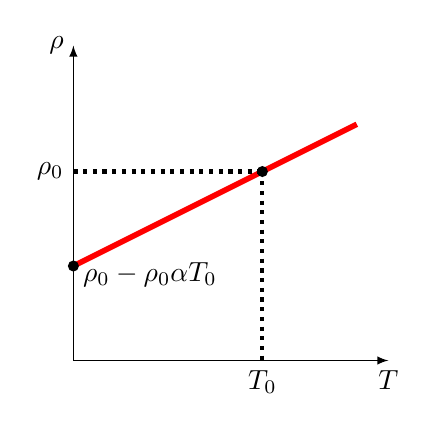
\begin{tikzpicture}[scale=0.4]
  \def\ro{6.0}
  \def\To{6.0}
  \def\alp{1.}
  
  \draw[-latex](0,0)--(10,0) node[below] {$T$};
  \draw[-latex](0,0)--(0,10) node[left] {$\rho$};
  \draw[color=red, line width=2pt] (0,3)--(9,7.5);
  \fill (6,6) circle(5pt);
  \fill (0,3) circle(5pt);
  \node[below=3pt, right] at (0,3) {$\rho_0-\rho_0\alpha T_0$} ;
  \draw[dotted,line width=1.5pt] (0,\ro) -- (\To,\ro);
  \node[left] at (0,\ro) {$\rho_0$} ;
  \draw[dotted,line width=1.5pt] (\To,\ro) -- (\To,0);
  \node[below] at (\To,0) {$T_0$} ;
  
\end{tikzpicture}
\captionof*{figure}{\textit{Resistivity as a function of temperature. It's a silly parametrization, because the slope is $\rho_0 \alpha$ instead of just $\alpha$.}}
}


%%%%%%%%%%%%%%%%%%%%%%%%%%%%%%
\subsubsection{Resistivity for a few materials}
\label{subsubsec:resistivityforafewmaterials}
\begin{frame}{Resistivity for a few materials}
\capfig{1}{figures/Current/table}{}

\end{frame}


%%%%%%%%%%%%%%%%%%%%%%%%%%%%%%
\subsection{Measuring resistance}
\label{subsec:measuringresistance}
\twocolframesf{Measuring resistance}
{
\begin{itemize}
\item Instead of a battery, we use a constant current source
\item We can measure the voltage across the resistor to find its resistance:
\begin{align*}
\Delta V = RI
\end{align*}
\item What is the resistance at room temperature ?
\end{itemize}
}
{
\begin{circuitikz}[]
\draw (0,0) [short] to (0,2)
      to [R,l_=$R$,i>=$I$] (4,2) 
      to [short,i>=$I$] (4,0) 
      to [current source,l^=$I$](0,0);  
\draw (1,2) [short,-*] to (1,3);
\draw (3,2) [short,-*] to (3,3);
\draw (1,3) [voltmeter] to (3,3);
\end{circuitikz}
\captionof*{figure}{\textit{Constant current source connected to a resistor. A voltmeter measures the voltage, $\Delta V$, across the resistor.}}
}



%%%%%%%%%%%%%%%%%%%%%%%%%%%%%%




%%%%%%%%%%%%%%%%%%%%%%%%%%%%%%
\subsection{Resistance versus temperature}
\label{subsec:resistanceversustemperature}
\twocolframesf{Resistance versus temperature}
{
What is the resistance
\begin{itemize}
\item At \SI{20}{\degree C} (room temperature)?
\item At \SI{0}{\degree C} (ice water)?
\item At \SI{100}{\degree C} (boiling water)?
\item At \SI{-196}{\degree C} (liquid nitrogen)?
\end{itemize}
}
{
\begin{circuitikz}[]
\draw (0,0) [short] to (0,2)
      to [R,l_=$R$,i>=$I$] (4,2) 
      to [short,i>=$I$] (4,0) 
      to [current source,l^=$I$](0,0);  
\draw (1,2) [short,-*] to (1,3);
\draw (3,2) [short,-*] to (3,3);
\draw (1,3) [voltmeter] to (3,3);
\end{circuitikz}
\captionof*{figure}{\textit{Constant current source connected to a resistor. A voltmeter measures the voltage, $\Delta V$, across the resistor.}}
}


%%%%%%%%%%%%%%%%%%%%%%%%%%%%%%



%%%%%%%%%%%%%%%%%%%%%%%%%%%%%%
\twocolframesf{Resistance versus temperature}
{
What is the resistance
\begin{itemize}
\item At \SI{-196}{\degree C} (liquid nitrogen)? \SI{1.32}{\Omega}
\item At \SI{0}{\degree C} (ice water)? \SI{6.0}{\Omega}
\item At \SI{20}{\degree C} (room temperature)? \SI{7.0}{\Omega}
\item At \SI{100}{\degree C} (boiling water)? \SI{8.0}{\Omega}
\end{itemize}
\begin{align*}
 R(T) &= R_0 \left[1+\alpha(T-T_0)\right]
\end{align*}
To get $\alpha$:
\begin{itemize}
\item Fit the data (the slope is $\alpha R_0$). Better method since it uses all the data.
\item Use the equation above at a given value of $T$.7
\end{itemize}
}
{
\capfig{1}{figures/Current/plot}{The resistivity is linear over \SI{300}{\degree C}!}

}

%%%%%%%%%%%%%%%%%%%%%%%%%%%%%%%%%



%%%%%%%%%%%%%%%%%%%%%%%%%%%%%%%%%%%%%%


\begin{frame}{Resistance vs Temperature}

\capfig{0.55}{figures/Current/RvsT}{Data from the previous lecture. Resistance is linear from \SI{-196}{\celsius} to \SI{100}{\celsius}!}

\end{frame}


%%%%%%%%%%%%%%%%%%%%%%%%%%%%%%







\section{Electrical Power}
\label{sec:electricalpower}
\title{Electrical Power}


%%%%%%%%%%%%%%%%%%%%%%%%%
\begin{frame}
\titlepage
\thispagestyle{empty}
\end{frame}




%%%%%%%%%%%%%%%%%%%%%%%%%%%%%%
\subsection{Batteries}
\label{subsec:batteries}
\twocolframesf{Batteries}
{
\begin{itemize}
\item Batteries have a positive ($+$) terminal and a negative terminal ($-$).
\item Batteries are characterized by the difference in electric potential between the positive and negative terminal that
they provide, e.g. a $\SI{9}{V}$ battery.
\item Most batteries exploit the properties of different materials to create an electrical potential difference.
\begin{itemize}
\item Often, this is done by exploiting the different affinities for materials to be dissolved in acid.
\end{itemize}
\end{itemize}
}
{
}

%%%%%%%%%%%%%%%%%%%%%%%%%%%%%%
%%%%%%%%%%%%% Defs for next figure
\def\proton at (#1,#2,#3){
\draw[fill=black,opacity=1] (#1,#2) circle (#3);
% a plus sign that scales
\draw[color=white] (#1-0.8*#3,#2) -- (#1+0.8*#3,#2);
\draw[color=white] (#1,#2-0.8*#3) -- (#1,#2+0.8*#3);
}

\def\ion at (#1,#2,#3){
\draw[fill=orange,opacity=1,draw=orange] (#1,#2) circle (#3);
% a plus sign that scales
\draw[color=white] (#1-0.8*#3,#2) -- (#1+0.8*#3,#2);
\draw[color=white] (#1,#2-0.8*#3) -- (#1,#2+0.8*#3);
}

\def\electron at (#1,#2,#3){
\fill[color=myred,opacity=1] (#1,#2) circle (#3);
% a minus sign that scales
\draw[color=white] (#1-0.8*#3,#2) -- (#1+0.8*#3,#2);
}

\subsection{The electric cell}
\label{subsec:theelectriccell}
\twocolframe{The electric cell}
{
\begin{itemize}
\item Zinc ``likes'' to be dissolved as an ion in acid.
\item The zinc ions leave their electrons behind in the electrode, making the zinc electrode negatively charged.
\item Electrons that are loosely bound in a carbon electrode are attracted into the electrolyte solution, leaving the carbon electrode positively charged.
\item Very quickly, the process stops as an equilibrium is reached, with a net electric potential difference between electrodes.
\end{itemize}
}
{ 
\begin{center}

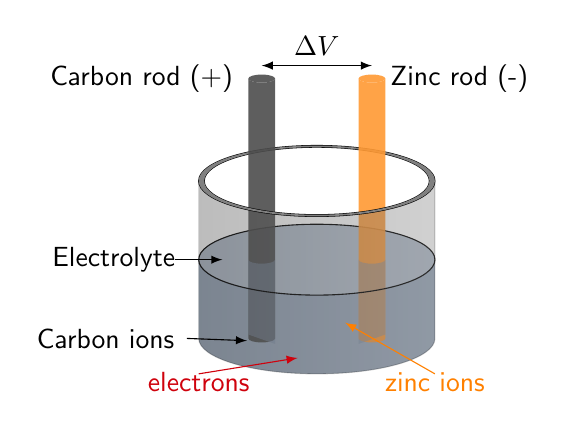
\begin{tikzpicture}[scale=1]
\tikzmath{
\Lou=2.0;
\Lw=1.0;
\Rou=1.5;
\dr=0.07;
\fac=0.3;
\Rd=0.17;
\Ld=3.3;
\xs=0.7;
\rp=0.1;
\re=0.05;
}  

\scalebox{1}{
%liquid:
  \fill[color=myblue!80,opacity=0.5] (-\Rou,0) arc (180:360:{\Rou} and {\fac*\Rou}) --  (\Rou,0)-- (\Rou, \Lw) arc (0:-180:{\Rou} and {\fac*\Rou}) -- (-\Rou,\Lw); 
  \fill[color=myblue!60, opacity=0.5] (\Rou,\Lw) arc (0:360:{\Rou} and {\fac*\Rou}) ;
 \draw[color=black] (\Rou,\Lw) arc (0:180:{\Rou} and {\fac*\Rou}) ;

%BACK RIM OF CONTAINER
  \draw[color=myblue!50, color=black, opacity=1, name path=A1] (\Rou,\Lou) arc (0:180:{\Rou} and {\fac*\Rou}) ;
  \draw[color=myblue!20, color=black, opacity=1, name path=B1] (\Rou-\dr,\Lou) arc (0:180:{\Rou-\dr} and {\fac*(\Rou-\dr)});
  \tikzfillbetween[of=A1 and B1]{gray}; 
  
%Rods:
  \fill[color=black!70,opacity=0.9] (-\Rd-\xs,0) arc (180:360:{\Rd} and {\fac*\Rd}) --  (\Rd-\xs,0)-- (\Rd-\xs, \Ld) arc (0:-180:{\Rd} and {\fac*\Rd}) -- (-\Rd-\xs,\Ld); 
  \fill[color=black!70, opacity=0.9] (\Rd-\xs,\Ld) arc (0:360:{\Rd} and {\fac*\Rd}) ;
  %\draw[color=black, dashed] (\Rd-\xs,\Lw) arc (0:360:{\Rd} and {\fac*\Rd}) ;
  \fill[color=myblue!50, opacity=0.5] (\Rd-\xs,\Lw) arc (0:-180:{\Rd} and {\fac*\Rd})  -- (-\xs-\Rd,\Lw-0.95) -- (-\xs+\Rd,\Lw-1.07);
    
  \fill[color=orange!80, opacity=0.9] (-\Rd+\xs,0) arc (180:360:{\Rd} and {\fac*\Rd}) --  (\Rd+\xs,0)-- (\Rd+\xs, \Ld) arc (0:-180:{\Rd} and {\fac*\Rd}) -- (-\Rd+\xs,\Ld); 
  \fill[color=orange!80, opacity=0.9] (\Rd+\xs,\Ld) arc (0:360:{\Rd} and {\fac*\Rd}) ;
  %\draw[color=orange, dashed] (\Rd+\xs,\Lw) arc (0:360:{\Rd} and {\fac*\Rd}) ;
  \fill[color=myblue!50, opacity=0.5] (\Rd+\xs,\Lw) arc (0:-180:{\Rd} and {\fac*\Rd})-- (\xs-\Rd,\Lw-1.07)  -- (\xs+\Rd,\Lw-0.95) ;
   
  \draw[color=black] (\Rou,\Lw) arc (0:-180:{\Rou} and {\fac*\Rou}) ;
   
%% particles
  \foreach \i in {1,3,...,7} {
   \proton at (-\xs-0.05,\i*\Ld/7-0.5,1.1*\rp)
   \electron at (\xs-0.07,\i*\Ld/7-0.5,1.1*\re)
  } 
  \foreach \i in {2,4,...,7} {
   \proton at (-\xs+0.07,\i*\Ld/7-0.5,0.9*\rp)
   \electron at (\xs+0.07,\i*\Ld/7-0.5,0.9*\re)
  } 
  
  \ion at (\xs-1.8*\Rd,1.3,0.9*\rp)
  \ion at (\xs-3*\Rd,1.2,0.9*\rp)
  \ion at (\xs-2*\Rd,\Ld/7-0.5,0.9*\rp)
  \ion at (\xs-2*\Rd,0.2,0.9*\rp)
  \ion at (\xs-3.2*\Rd,\Ld/7-0.7,\rp)
  \ion at (\xs-4*\Rd,0,1.1*\rp)
  \ion at (\xs-4.5*\Rd,\Ld/7-0.5,1.1*\rp)
  
  \electron at (-\xs+1.2*\Rd,\Ld/7-0.5,0.9*\re)
  \electron at (-\xs+2*\Rd,0.2,0.9*\re)
  \electron at (-\xs+2*\Rd,0.6,0.9*\re)
  \electron at (-\xs+1.7*\Rd,1.2,1.1*\re)
  \electron at (-\xs+2.8*\Rd,\Ld/7-0.7,\re)
  \electron at (-\xs+3*\Rd,0.4,1.1*\re)
  \electron at (-\xs+2.5*\Rd,\Ld/7,\re)
          
%front of container:
  \fill[left color=gray,right color=gray!20,shading=axis,opacity=0.2, draw=black] (-\Rou,0) arc (180:360:{\Rou} and {\fac*\Rou}) --  (\Rou,0)-- (\Rou, \Lou) arc (0:-180:{\Rou} and {\fac*\Rou}) -- (-\Rou,\Lou); 
  \draw[color=myblue!50, color=black, opacity=1, name path=A2] (\Rou,\Lou) arc (0:-180:{\Rou} and {\fac*\Rou}) ;
  \draw[color=myblue!20, color=black, opacity=1, name path=B2] (\Rou-\dr,\Lou) arc (0:-180:{\Rou-\dr} and {\fac*(\Rou-\dr)});
  \tikzfillbetween[of=A2 and B2]{gray}; 
 
 
 \node[above, left=2pt] at (-\Rd-\xs,\Ld){{Carbon rod (+)}};
 \node[above, right=8pt] at (-\Rd+\xs,\Ld){{Zinc rod (-)}};
 \draw[color=myred,-latex](-\Rou,-0.6*\Rou/2)  node[below=-4pt] {{electrons}}  -- (-\xs+2.8*\Rd,\Ld/7-0.7,\re);
 \draw[-latex](-1.1*\Rou,0)  node[left=1pt] {{Carbon ions}}  -- (-\xs-1.1*\Rd,\Ld/7-0.5);
 \draw[color=orange,-latex](\Rou,-0.6*\Rou/2)  node[below=-4pt] {{zinc ions}}  -- (\xs-2*\Rd,0.2);
 \draw[-latex] (-1.2*\Rou,\Lou/2) -- (-0.8*\Rou,\Lou/2);
 \node[left=5pt] at (-\Rou,\Lou/2) {{Electrolyte}};  
 \draw[latex-latex] (-\xs,1.05*\Ld) -- (\xs,1.05*\Ld) node[above,midway] {{$\Delta V$}}; 
 }
\end{tikzpicture}
\captionof*{figure}{\textit{An electric cell made with an electrolyte, such as $H_2SO_4$ (sulfuric acid) and two metals.}}
\end{center}
}


%%%%%%%%%%%%%%%%%%%%%%%%%%%%%%




%%%%%%%%%%%%%%%%%%%%%%%%%%%%%%
\subsection{Power dissipated in a resistor}
\label{subsec:powerdissipatedinaresistor}
\begin{frame}{Power dissipated in a resistor}
\capfig{0.5}{figures/Current/resistor}{An electron losing energy in a resistor.}
\begin{itemize}
\item As electrons move through a resistor, they collide with atoms therein. 
\item The electric field does work on the electrons, which is then converted into heating up the resistor – no net work is done on the electrons
(their average speed is unchanged).
\item The rate at which kinetic energy of the electrons is converted into thermal energy is called the “electric(al) power” dissipated in a resistor.
\end{itemize}

\end{frame}


%%%%%%%%%%%%%%%%%%%%%%%%%%%%%%
\subsection{Electric power}
\label{subsec:electricpower}
\twocolframesf{Electric power}
{
\begin{itemize}
\item Consider the energy that 1 charge q must deposit in the resistor. The total energy available is the change in potential energy:
\begin{align*}
\Delta U = q \Delta V
\end{align*}
\item If we have many charges going through the resistor, each charge deposits energy E in the form of heat. Then, it makes more sense to define how much
\textit{energy per unit time} is deposited in the resistor (which we call power):
\begin{align*}
P=\frac{d}{dt}\Delta U=\frac{d}{dt}q\Delta V = \frac{dq}{dt}\Delta V = I\Delta V
\end{align*}
\end{itemize}
}
{\capfig{1}{figures/Current/bigresistor}{A potential difference across a resistor.}}



%%%%%%%%%%%%%%%%%%%%%%%%%%%%%%
\twocolframesf{Some sloppy notation}
{
\vspace{-0.25cm}
\begin{itemize}
\item We apply a potential difference across a resistor, $\Delta V$.
\item Ohm’s Law tells us how this relates to current and resistance:
\begin{align*}
\Delta V = RI
\end{align*}
\item It is so patently clear that this only makes sense for a potential difference, that all the cool people just drop the $\Delta$ and write:
\begin{align*}
V = RI
\end{align*}
Up to you if you are comfortable with this... The $V$ in the equation above is the \textit{difference} in potential between $B$ and $A$. 
\end{itemize}
}
{\capfig{1}{figures/Current/bigresistor}{A potential difference across a resistor.}}


%%%%%%%%%%%%%%%%%%%%%%%%%%%%%%
\begin{frame}{Electric power}
\begin{itemize}
\item If we have a voltage $V$, across a resistor $R$, and current $I$, then the rate at which heat is dissipated into the resistor is given by:
\begin{align*}
P= I V
\end{align*}
\item Using Ohm’s Law to get rid of $I$ or $V$, we can rewrite this as:
\begin{align*}
P &= I^2R \;\;\;\;\text{(say, we know the current through a resistor)}\\
P &= \frac{V^2}{R} \;\;\;\;\text{(say, we know the voltage across a resistor)}
\end{align*}
\end{itemize}

\end{frame}



%%%%%%%%%%%%%%%%%%%%%%%%%%%%%%
\subsection{Household appliances}
\label{subsec:householdappliances}
\twocolframesf{Household appliances}
{
\begin{itemize}
\item Household appliances are designed such that they will work with a fixed voltage difference (\SI{120}{V} in North America).
\item Often appliances have specifications about how much power they
use:
\begin{itemize}
\item \SI{1500}{W} microwave.
\item \SI{60}{W} lightbulb.
\item \SI{1200}{W} hair dryer.
\end{itemize}
\item[$\rightarrow$]These specifications are always assuming that they have a constant
voltage applied to them (\SI{120}{V} in North America).
\end{itemize}
}
{
\vspace{-1cm}
\capfig{0.3}{figures/Current/bulb}{\tiny{\url{https://commons.wikimedia.org/wiki/File:Gluehlampe_01_KMJ.jpg}}}

\vspace{-1cm}
\capfig{0.5}{figures/Current/hairdryer}{\tiny{\url{https://www.ebay.ca/itm/333729494226}}}
}


%%%%%%%%%%%%%%%%%%%%%%%%%%%%%%



%%%%%%%%%%%%%%%%%%%%%%%%%%%%%%
\subsection{AC voltage and current}
\label{subsection:ac}
\begin{frame}{Alternating current/voltage - Why?!}
\begin{itemize}
\item Electricity (electric power) is useful, right?
\item So we need efficient ways to produce and transmit it!
\item We can generate DC current (giant batteries), but it’s not efficient or practical for the amount of energy that our society uses.
\item It’s very easy to generate AC current (or AC voltage) using a generator.
\end{itemize}

\end{frame}


%%%%%%%%%%%%%%%%%%%%%%%%%%%%%%
\twocolframesf{Electric generator}
{
\begin{itemize}
\item In a few weeks, you will learn about electromagnetic induction:
\begin{itemize}
\item If we change the magnetic flux through a coil, we can generate a voltage.
\end{itemize}
\item If we rotate a coil in a fixed magnetic field, we will generate a sinusoidal voltage:
\begin{align*}
V = V_0\sin(\omega t)
\end{align*}
\item Easy to build turbines (things that spin when we run water or hot gases through
them)
\begin{itemize}
\item Convert mechanical or thermal energy into electric potential energy
\end{itemize} 
\end{itemize}
}
{
\vspace{-1cm}
\capfig{0.5}{figures/Current/generator}{\tiny{\url{https://www.texasgateway.org/resource/65-electric-generators}}}

\vspace{-1cm}
\capfig{0.5}{figures/Current/dam}{\tiny{\url{https://energyeducation.ca/encyclopedia/Hydroelectric_facility}}}

}


%%%%%%%%%%%%%%%%%%%%%%%%%%%%%%
\twocolframe{AC Voltage and current}
{
\begin{itemize}
\item Ohm’s law still true, so across a resistor with sinusoidal voltage:
\begin{align*}
V &= V_0\sin(\omega t)\\
V &= RI\\
I &=\frac{V}{R}=\frac{V_0}{R}\sin(\omega t)=I_0\sin(\omega t)
\end{align*}
\item The average current/voltage is 0. 
\end{itemize}
}
{
\centering
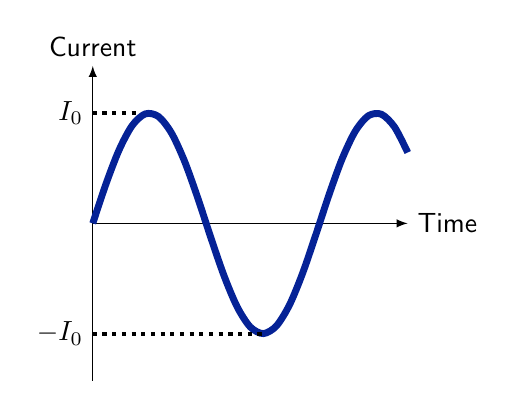
\begin{tikzpicture}[scale=0.4]
  \def\Io{3.5}
  
  \draw[-latex](0,0)--(10,0) node[right] {Time};
  \draw[-latex](0,-5)--(0,5) node[above] {Current};
  \draw[color=myblue2, line width=2.5pt, domain=0:10, smooth, variable=\x,]  plot (\x,{\Io*sin(50*\x)});
  \draw[dotted,line width=1.5pt] (0,\Io) -- (1.5,\Io);
  \node[left] at (0,\Io) {$I_0$} ;
  \draw[dotted,line width=1.5pt] (0,-\Io) -- (5.5,-\Io);
  \node[left] at (0,-\Io) {$-I_0$} ;  
\end{tikzpicture}
\captionof*{figure}{\textit{Alternating current, from negative to positive.}}

}

%%%%%%%%%%%%%%%%%%%%%%%%%%%%%%
\subsection{Power dissipated in a resistor with AC current}
\label{subsubsec:powerdissipatedinaresistorwithaccurrent}
\twocolframe{Power dissipated in a resistor with AC current}
{
\vspace{-0.25cm}
\begin{itemize}
\item If the current is given by:
\begin{align*}
I(t)=I_0\sin(\omega t)
\end{align*}
\item the instantaneous power dissipated in the resistor (at some time, $t$) is:
\begin{align*}
P(t)=I^2(t)R=I^2_0\sin^2(\omega t)R
\end{align*}
\item The average power is non-zero:
\begin{align*}
\bar P=I^2_0R\overline{\sin^2(\omega t)}=\frac{1}{2}I^2_0 R
\end{align*}
\end{itemize}
(The average value of $\sin^2(\omega t)$ over one period is $\frac{1}{2}$.)
}
{
\centering
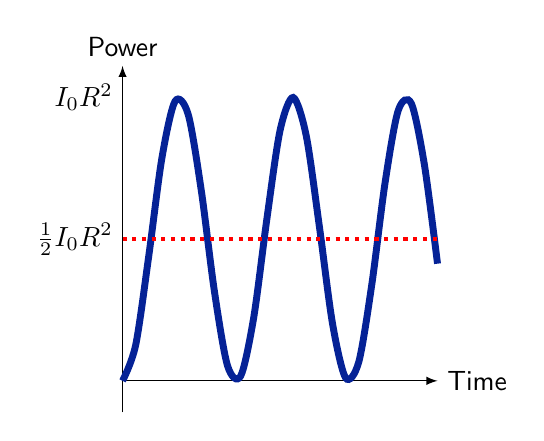
\begin{tikzpicture}[scale=0.4]
  \def\Io{3}
  \def\Res{1.0}
  
  \draw[-latex](0,0)--(10,0) node[right] {Time};
  \draw[-latex](0,-1)--(0,10) node[above] {Power};
  \draw[color=myblue2, line width=2.5pt, domain=0:10, smooth, variable=\x,]  plot (\x,{\Res*\Io*\Io*sin(50*\x)*sin(50*\x)});
  \draw[dotted, color=red,line width=1.5pt] (0,0.5*\Io*\Io) -- (10,0.5*\Io*\Io);
  \node[left] at (0,0.5*\Io*\Io) {$\frac{1}{2}I_0R^2$} ; 
  \node[left] at (0,\Io*\Io) {$I_0R^2$} ; 
\end{tikzpicture}
\captionof*{figure}{\textit{With alternating current, the instaneous dissipated power is always greater than zero (makes sense).}}

}



%%%%%%%%%%%%%%%%%%%%%%%%%%%%%%
\subsection{RMS current}
\label{subsec:rmscurrent}
\begin{frame}{RMS Current}
\vspace{-0.25cm}
\begin{itemize}
\item  For sinusoidal current, with maximum amplitude $I_0$, we can write the average dissipated power as:
\begin{align*}
\bar P=\frac{1}{2}I^2_0 R
\end{align*}
\item Would like to have some sort of “effective” current, $I_{eff}$, so that we can use the ``usual'' formula for power:
\begin{align*}
\bar P=I^2_{eff}R
\end{align*}
\item This works if we introduce an ``efective current'', $I_{eff}$, called the RMS current:
\begin{align*}
I^2_{eff}&=\frac{1}{2}I^2_0\\
\therefore I_{eff} &= \frac{1}{\sqrt 2} I_0 = I_{rms}
\end{align*}
\end{itemize}
$I_{rms}$ is the average value of the square of the current, the \textit{square root of the mean of the squared current}: 
$I^2_{rms}=I^2_0\overline{\sin^2(\omega t)}=\frac{1}{2}I^2_0$
\end{frame}


%%%%%%%%%%%%%%%%%%%%%%%%%%%%%%
\subsubsection{RMS voltage}
\label{subsubsec:rmsvoltage}
\begin{frame}{RMS Current and voltage}
\begin{itemize}
\item We can define \textit{RMS values} of the current and voltage:
\begin{align*}
I_{rms}=\frac{1}{\sqrt 2} I_0 \;\;\;\; V_{rms}=\frac{1}{\sqrt 2} V_0
\end{align*}
\item This allows us to easily calculate the average power dissipated by a resistor when it has AC voltage (current) across (through) it, using the RMS values:
\begin{align*}
V_{RMS}=RI_{rms} \;\;\;\; \bar P=I^2_{rms}R\;\;\;\; \bar P=I_{rms}V_{rms}\;\;\;\; \bar P=\frac{V^2_{rms}}{R}
\end{align*}
\item Remember, the \textit{instantaneous power} changes as a function of time, so it’s more useful to think about the average power that our appliances use (e.g. how much will it cost to have a \SI{100}{W} light bulb on all the time).
\end{itemize}
\end{frame}

%%%%%%%%%%%%%%%%%%%%%%%%%%%%%%%%%%%%%%%



%%%%%%%%%%%%%%%%%%%%%%%%%%%%%



%%%%%%%%%%%%%%%%%%%%%%%%%%%%%%



%%%%%%%%%%%%%%%%%%%%%%%%%%%%%%%



%%%%%%%%%%%%%%%%%%%%%%%%%%%%%%%%%%%



%%%%%%%%%%%%%%%%%%%%%%%%%%%%%%%%%%



\end{document}

